\documentclass{beamer}
\usetheme{Singapore}
\usepackage[round,sort]{natbib}
\usepackage{tikz}
\usetikzlibrary{arrows,decorations.pathmorphing,backgrounds,fit,positioning,shapes.symbols,chains}
\usepackage{adjustbox}
\usepackage{verbatim}
\usepackage{graphicx}
\usepackage{hyperref}

\usepackage{tabu}
\hypersetup{
    colorlinks=true,
    linkcolor=blue,
    filecolor=cyan,      
    urlcolor=cyan,
    citecolor=blue,
}

\graphicspath{ {sms2017-presentation-images/} }

\title{Heterogeneity in Knowledge Flows of Regions: Impact on Invention Quality}
%\subtitle{QE Research Paper}
\author{Ashwin Iyenggar}
\institute[Indian Institute of Management Bangalore] 
{
  Doctoral Student, Strategy Area\\
  Indian Institute of Management Bangalore
}
\date{30 November, 2017 \\ SMS 27th Annual Conference, Houston}
\subject{Heterogeneity in Knowledge Flows of Regions: Impact on Invention Quality}

% \pgfdeclareimage[height=0.5cm]{university-logo}{university-logo-filename}
% \logo{\pgfuseimage{university-logo}}

\AtBeginSubsection[]
{
  \begin{frame}<beamer>{Outline}
    \tableofcontents[currentsection,currentsubsection]
  \end{frame}
}

\begin{document}

\begin{frame}
  \titlepage
\end{frame}

\begin{frame}{Outline}
  \tableofcontents
  % You might wish to add the option [pausesections]
\end{frame}


\section{Motivation}

\begin{frame}{Prior art on knowledge flows}{Patent citation analysis}
\textbf{Economic Geography Literature}
\begin{itemize}
\item{Knowledge spillovers are localized \citep*{Jaffe1993}}
\item{Innovation is more spatially concentrated than is production \citep{Feldman1994a}}
\end{itemize}

\textbf{International Business Literature}
\begin{itemize}
\item{Firms profit from offshoring R\&D by leveraging better organizational linkages \citep*{Zhao2006}}
\item{Subsidiary - MNC parent flows are as strong as MNC parent - Subsidiary knowledge flows \citep{Singh2007}}
\end{itemize}
\end{frame}

\begin{frame}{Knowledge flows as outcome of search?}{Region and firm boundaries}
\begin{figure}[h!]
\begin{centering}
  \includegraphics[width=0.6\textwidth]{2x2old}
  \caption{Categories of knowledge flows}
   \label{fig:2x2old}
\end{centering}
\end{figure}
\end{frame}

\begin{frame}{Research Question}{}

\textit{How do the \textbf{nature} of knowledge flows in a region affect the \textbf{quality} of inventions generated in the region?}

\end{frame}

\begin{frame}{Summary of Preliminary Findings}{}
\begin{itemize}
\item{Localized knowledge flows do not seem to improve invention quality}
\item{Geographical diversification is seen to improve invention quality}
\item{Results differ between applicant only citations data and applicant and examiner citations dataset echoing concerns raised by \cite{Alcacer2006a}}
\item{Much additional research required to distill any stylized facts on the impact of geography and firm boundaries on invention quality}
\end{itemize}
\end{frame}

\section{Literature Review}
\begin{frame}{On the Nature of Knowledge Spillovers}{}
\begin{itemize}
\item{Rent Spillovers vs. Pure Spillovers \citep{Griliches1979}}
\item{Knowledge as a private good and a public good \citep{Arrow1962}}
\item{Knowledge flows are invisible \citep{Krugman1991a}}
\item{Knowledge flows sometimes leave a paper trail in the form of patent citations \citep{Jaffe1993}}
\end{itemize}
\end{frame}

\begin{frame}{On the Localization of Knowledge Spillovers}{}
\begin{itemize}
\item{Proximity is beneficial due to lower costs of collaboration, opportunities for serendipitous encounters}
\item{Tacit knowledge is not easily transferred across long distances}
\item{Institutions and Regional innovation systems contribute to localization of knowledge flows}
\item{Related variety \citep*{Boschma2009, Frenken2007, Jacobs1969} in urban clusters promotes generation of new ideas}
\end{itemize}
\end{frame}

\begin{frame}{On Knowledge Flows across Countries}{}
\begin{itemize}
\item{Political borders may constrain flows of knowledge \citep{Singh2013}}
\item{Inventor mobility improves innovation outcomes \citep{Alnuaimi2012a}}
\item{MNC subsidiary location choices influenced by regional innovation systems \citep{Andersen2005}, organizational linkages \citep{Zhao2006}, and higher independence and ownership \citep{Pearce1999}}
\end{itemize}
\end{frame}

\section{Theory and Hypotheses}
\begin{frame}{Invention quality at the independent research center}{}
\begin{figure}[h]
\centering
\begin{adjustbox}{width=\textwidth}
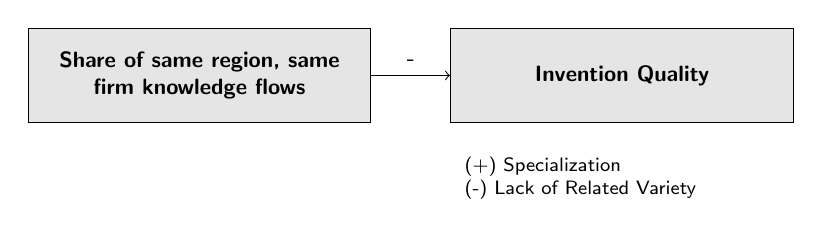
\begin{tikzpicture}
[node distance = 1cm, auto,font=\footnotesize,
every node/.style={node distance=3cm},
comment/.style={rectangle, inner sep= 5pt, text width=4cm, node distance=0.25cm, font=\scriptsize\sffamily},
force/.style={rectangle, draw, fill=black!10, inner sep=5pt, text width=4cm, text badly centered, minimum height=1.2cm, font=\bfseries\footnotesize\sffamily}]
\node [force] (quality) {Invention Quality};
\node [force, left=1cm of quality] (share) {Share of same region, same firm knowledge flows};

\draw[->] (share) edge node{-} (quality);
\node [comment, below=0.25 of quality] (comment) {(+) Specialization\\
(-) Lack of Related Variety};
\end{tikzpicture}
\end{adjustbox}
\caption{Hypothesized relationship of knowledge flows within an independent research center on invention quality}
\label{figure:q1}
\end{figure}
\end{frame}

\begin{frame}{Invention quality in a cluster}{}
\begin{figure}[h]
\centering
\begin{adjustbox}{width=\textwidth}
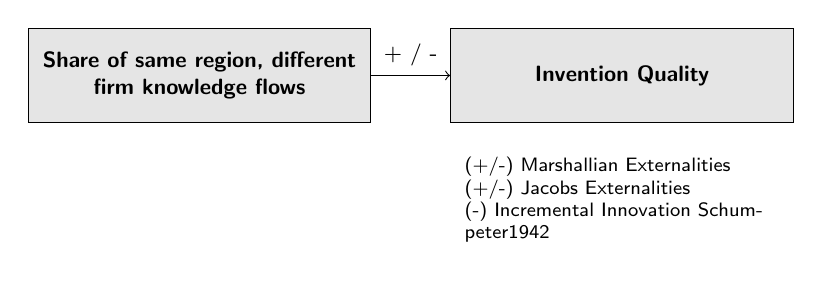
\begin{tikzpicture}
[node distance = 1cm, auto,font=\footnotesize,
every node/.style={node distance=3cm},
comment/.style={rectangle, inner sep= 5pt, text width=4cm, node distance=0.25cm, font=\scriptsize\sffamily},
force/.style={rectangle, draw, fill=black!10, inner sep=5pt, text width=4cm, text badly centered, minimum height=1.2cm, font=\bfseries\footnotesize\sffamily}]
\node [force] (quality) {Invention Quality};
\node [force, left=1cm of quality] (share) {Share of same region, different firm knowledge flows};
\node [comment, below=0.25 of quality] (comment) {(+/-) Marshallian Externalities\\
(+/-) Jacobs Externalities \\ (-) Incremental Innovation \citep{Schumpeter1942}};
\draw[->] (share) edge node{+ / -} (quality);
\end{tikzpicture}
\end{adjustbox}
\caption{Hypothesized relationship of knowledge flows within a cluster on invention quality}
\label{figure:q1}
\end{figure}
\end{frame}

\begin{frame}{Invention quality under geographical diversification}{}
\begin{figure}[h]
\centering
\begin{adjustbox}{width=\textwidth}
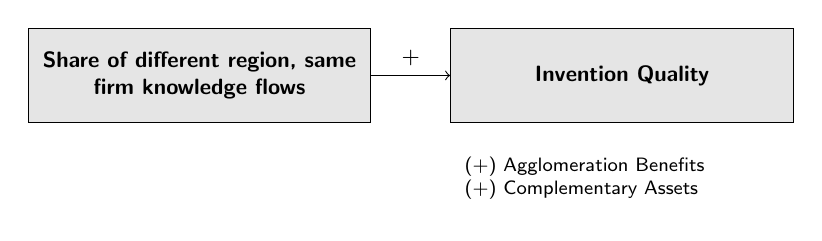
\begin{tikzpicture}
[node distance = 1cm, auto,font=\footnotesize,
every node/.style={node distance=3cm},
comment/.style={rectangle, inner sep= 5pt, text width=4cm, node distance=0.25cm, font=\scriptsize\sffamily},
force/.style={rectangle, draw, fill=black!10, inner sep=5pt, text width=4cm, text badly centered, minimum height=1.2cm, font=\bfseries\footnotesize\sffamily}]
\node [force] (quality) {Invention Quality};
\node [force, left=1cm of quality] (share) {Share of different region, same firm knowledge flows};
\node [comment, below=0.25 of quality] (comment) {(+) Agglomeration Benefits\\
(+) Complementary Assets};
\draw[->] (share) edge node{+} (quality);
\end{tikzpicture}
\end{adjustbox}
\caption{Hypothesized relationship of knowledge flows under geographical diversification on invention quality}
\label{figure:q1}
\end{figure}
\end{frame}

\begin{frame}{Invention quality under diffusion}{}
\begin{figure}[h]
\centering
\begin{adjustbox}{width=\textwidth}
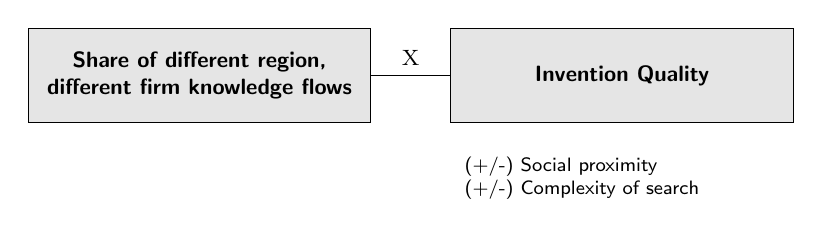
\begin{tikzpicture}
[node distance = 1cm, auto,font=\footnotesize,
every node/.style={node distance=3cm},
comment/.style={rectangle, inner sep= 5pt, text width=4cm, node distance=0.25cm, font=\scriptsize\sffamily},
force/.style={rectangle, draw, fill=black!10, inner sep=5pt, text width=4cm, text badly centered, minimum height=1.2cm, font=\bfseries\footnotesize\sffamily}]
\node [force] (quality) {Invention Quality};
\node [force, left=1cm of quality] (share) {Share of different region, different firm knowledge flows};
\node [comment, below=0.25 of quality] (comment) {(+/-) Social proximity\\
(+/-) Complexity of search };
\draw[-] (share) edge node{X} (quality);
\end{tikzpicture}
\end{adjustbox}
\caption{Hypothesized relationship of knowledge flows under diffusion on invention quality}
\label{figure:q1}
\end{figure}
\end{frame}



\section{Data and Method}
\begin{frame}{Geographic Mapping}{San Jose}
\begin{figure}[h!]
\begin{centering}
  \includegraphics[width=0.6\textwidth]{SanJose}
  \caption{Geographic Definition of San Jose, CA}
   \label{fig:SanJose}
\end{centering}
\end{figure}
\end{frame}

\begin{frame}{Summary Statistics}{Applicant only citations}
\centering
\adjustbox{max height=\dimexpr\textheight-5.5cm\relax,
           max width=\textwidth}{
\begin{tabular}{l c c  c}\hline\hline
\multicolumn{1}{c}{\textbf{Variable}} & \textbf{Mean}
 & \textbf{Std. Dev.} & \textbf{N}\\ \hline
Citations Received & 1630.527 & 8200.133  & 9358\\
Non-Self Citations Received & 917.342 & 4958.117  & 9358\\
Self Citations Received & 248.898 & 1312.542  & 9358\\
Share Citations Made[Same Region, Same Assignee] & 0.013 & 0.034  & 9358\\
Share Citations Made[Same Region, Different Assignee] & 0.013 & 0.039  & 9358\\
Share Citations Made[Different Region, Same Assignee] & 0.038 & 0.076  & 9358\\
Share Citations Made[Different Region, Different Assignee] & 0.509 & 0.2  & 9358\\
Share Citations Made[Other] & 0.428 & 0.202  & 9358\\
Share Citations Made[Same Region] & 0.026 & 0.054  & 9358\\
Share Citations Made[Same Assignee] & 0.051 & 0.087  & 9358\\
Log (Total Citations Made) & 4.92 & 2.411  & 9358\\
Log (Num Patents) & 3.719 & 1.954  & 9358\\
Log (Patent Pool Size) & 6.496 & 2.048  & 9358\\
\hline\end{tabular}
}
\end{frame}

\begin{frame}{Methodology}{}
\begin{itemize}
\item{Data Source: Patents from USPTO, source: patentsview.org}
\item{Data Source: Regions using Remote Sensing Data, source: naturalearthdata.com}
\item{Unit of Analysis: Region-Year}
\item{Dependent Variables: Total Citations Received, Non-Self Citations Received}
\item{Independent Variables: Share of citations made within/outside region, within/outside assignee}
\item{Control Variables: Technology subcategories \citep*{Hall2001a}, Region fixed effects, Year effects}
\item{Estimation Method: Negative Binomial}
\end{itemize}
\end{frame}


\begin{frame}{Results}{Applicant only citations}
\centering
\adjustbox{max height=\dimexpr\textheight-5.5cm\relax,
           max width=\textwidth}{
\begin{tabular}{l*{6}{c}} \hline\hline
                &\multicolumn{1}{c}{(1)}&\multicolumn{1}{c}{(2)}&\multicolumn{1}{c}{(3)}&\multicolumn{1}{c}{(4)}&\multicolumn{1}{c}{(5)}&\multicolumn{1}{c}{(6)}\\
                &\multicolumn{1}{c}{Total}&\multicolumn{1}{c}{Total}&\multicolumn{1}{c}{Total}&\multicolumn{1}{c}{Non-Self}&\multicolumn{1}{c}{Non-Self}&\multicolumn{1}{c}{Non-Self}\\
                &\multicolumn{1}{c}{Citations}&\multicolumn{1}{c}{Citations}&\multicolumn{1}{c}{Citations}&\multicolumn{1}{c}{Citations}&\multicolumn{1}{c}{Citations}&\multicolumn{1}{c}{Citations}\\
                 &\multicolumn{1}{c}{Received}&\multicolumn{1}{c}{Received}&\multicolumn{1}{c}{Received}&\multicolumn{1}{c}{Received}&\multicolumn{1}{c}{Received}&\multicolumn{1}{c}{Received}\\
\hline
Share Citations Made[Same Region, Same Assignee]&   -0.125&   -0.156&  -0.0437&  -0.0698&  -0.0575&   -0.113\\
                &  (0.372)&  (0.468)&  (0.809)&  (0.613)&  (0.782)&  (0.560)\\
Share Citations Made[Same Region, Different Assignee]&  -0.0501&   -0.250&   0.0494&    0.214&   0.0341&    0.267\\
                &  (0.677)&  (0.305)&  (0.704)&  (0.052)&  (0.889)&  (0.035)\\
Share Citations Made[Different Region, Same Assignee]&    0.260&    0.316&    0.326&    0.215&    0.209&    0.247\\
                &  (0.002)&  (0.015)&  (0.003)&  (0.013)&  (0.105)&  (0.040)\\
Share Citations Made[Different Region, Different Assignee]&  0.00251&   0.0382&   0.0123&   0.0426&   0.0336&   0.0615\\
                &  (0.933)&  (0.383)&  (0.760)&  (0.160)&  (0.447)&  (0.143)\\
Log (Total Citations Made)&   0.0194&   0.0126&   0.0220&   0.0131&  0.00662&   0.0152\\
                &  (0.000)&  (0.031)&  (0.000)&  (0.002)&  (0.258)&  (0.012)\\
Log (Num Patents)&    0.788&    0.860&    0.830&    0.799&    0.826&    0.849\\
                &  (0.000)&  (0.000)&  (0.000)&  (0.000)&  (0.000)&  (0.000)\\
Log (Patent Pool Size)&   -0.124&   -0.303&   -0.110&  -0.0871&   -0.157&   -0.108\\
                &  (0.000)&  (0.000)&  (0.000)&  (0.000)&  (0.000)&  (0.000)\\
Constant        &   -0.911&    0.510&   -1.368&   -1.296&   -0.557&   -1.677\\
                &  (0.000)&  (0.002)&  (0.000)&  (0.000)&  (0.002)&  (0.000)\\
\hline
Observations    &     9358&     3974&     5384&     9037&     3868&     5169\\
Groups          &     1359&      539&      820&     1255&      503&      752\\
Sample&All &U.S. &Non-U.S.&All &U.S. &Non-U.S. \\
          &Locations &Locations&Locations&Locations &Locations&Locations \\\hline\hline
\multicolumn{7}{l}{\footnotesize \textit{p}-values in parentheses}\\
\multicolumn{7}{l}{\footnotesize All models include region fixed effects, year dummies and technology subcategory controls}\\
\end{tabular}
}
\end{frame}

\section{Future Work}
\begin{frame}{Addressing Potential Issues}{Applicant and Examiner Citations}
\centering
\adjustbox{max height=\dimexpr\textheight-5.5cm\relax,
           max width=\textwidth}{
\begin{tabular}{l*{6}{c}} \hline\hline
                &\multicolumn{1}{c}{(1)}&\multicolumn{1}{c}{(2)}&\multicolumn{1}{c}{(3)}&\multicolumn{1}{c}{(4)}&\multicolumn{1}{c}{(5)}&\multicolumn{1}{c}{(6)}\\
                &\multicolumn{1}{c}{Total}&\multicolumn{1}{c}{Total}&\multicolumn{1}{c}{Total}&\multicolumn{1}{c}{Non-Self}&\multicolumn{1}{c}{Non-Self}&\multicolumn{1}{c}{Non-Self}\\
                &\multicolumn{1}{c}{Citations}&\multicolumn{1}{c}{Citations}&\multicolumn{1}{c}{Citations}&\multicolumn{1}{c}{Citations}&\multicolumn{1}{c}{Citations}&\multicolumn{1}{c}{Citations}\\
                 &\multicolumn{1}{c}{Received}&\multicolumn{1}{c}{Received}&\multicolumn{1}{c}{Received}&\multicolumn{1}{c}{Received}&\multicolumn{1}{c}{Received}&\multicolumn{1}{c}{Received}\\
\hline
Share Citations Made[Same Region, Same Assignee]&    0.818&    0.463&    1.258&    1.403&    1.294&    1.641\\
                &  (0.000)&  (0.126)&  (0.000)&  (0.000)&  (0.000)&  (0.000)\\
Share Citations Made[Same Region, Different Assignee]&   -0.846&   -1.158&   -0.444&   0.0468&   -0.433&    0.227\\
                &  (0.004)&  (0.006)&  (0.268)&  (0.885)&  (0.374)&  (0.606)\\
Share Citations Made[Different Region, Same Assignee]&    0.652&    0.365&    0.843&    1.139&    0.792&    1.192\\
                &  (0.000)&  (0.055)&  (0.000)&  (0.000)&  (0.001)&  (0.000)\\
Share Citations Made[Different Region, Different Assignee]&   0.0517&    0.230&    0.109&    0.994&    1.354&    0.920\\
                &  (0.195)&  (0.000)&  (0.037)&  (0.000)&  (0.000)&  (0.000)\\
Log (Total Citations Made)&   0.0656&   0.0290&   0.0858&  -0.0349&  -0.0813&   0.0387\\
                &  (0.000)&  (0.031)&  (0.000)&  (0.000)&  (0.000)&  (0.005)\\
Log (Num Patents)&    0.730&    0.820&    0.755&    0.845&    0.919&    0.805\\
                &  (0.000)&  (0.000)&  (0.000)&  (0.000)&  (0.000)&  (0.000)\\
Log (Patent Pool Size)&  -0.0982&   -0.273&   -0.102&  -0.0571&   -0.145&  -0.0743\\
                &  (0.000)&  (0.000)&  (0.000)&  (0.000)&  (0.000)&  (0.000)\\
Constant        &   -0.185&    1.003&   -0.547&   -1.000&   -0.390&   -1.312\\
                &  (0.000)&  (0.000)&  (0.000)&  (0.000)&  (0.000)&  (0.000)\\
\hline
Observations    &    18102&     6850&    11252&    17730&     6749&    10981\\
Groups          &     2006&      631&     1375&     1896&      610&     1286\\
Sample&All &U.S. &Non-U.S.&All &U.S. &Non-U.S. \\
          &Locations &Locations&Locations&Locations &Locations&Locations \\\hline\hline
\multicolumn{7}{l}{\footnotesize \textit{p}-values in parentheses}\\
\multicolumn{7}{l}{\footnotesize All models include region fixed effects, year dummies and technology subcategory controls}\\
\end{tabular}
}
\end{frame}

\begin{frame}{Limitations}{}
\begin{itemize}
\item{The use of patent citations as a measure of knowledge flows may be subject to error \citep{Arora2017a}}
\item{Any systematic biases in our definition of regions (Urban Centers from Natural Earth Data) can create biases in measures of knowledge flows}
\end{itemize}
\end{frame}

\begin{frame}{Future Work}{}
\begin{itemize}
\item{Examine the effects of search on technology domain \citep{Rosenkopf2001}}
\item{Investigate the effect on alternate outcomes, e.g., breakthrough inventions}
\item{Identify the mechanisms underlying the impact of knowledge flows on invention quality}
\end{itemize}
\end{frame}

\bibliography{/Users/aiyenggar/code/bibliography/aiyenggar}
\bibliographystyle{ai-amjlike}

\end{document}

\begin{comment}

\begin{frame}{Geographic Mapping}{Bangalore}
\begin{figure}[h!]
\begin{centering}
  \includegraphics[width=0.7\textwidth]{Bangalore}
  \caption{Geographic Definition of Bangalore}
   \label{fig:Bangalore}
\end{centering}
\end{figure}
\end{frame}


\begin{figure}[h]
\begin{centering}
  \includegraphics[width=\textwidth]{TelAviv}
  \caption{Geographic Definition of Tel Aviv-Yafo}
   \label{fig:TelAviv}
\end{centering}
\end{figure}
\end{comment}

